\chapter{Our Proposal}

Our ultimate goal is to build a comprehensive and universal framework for computer-aided drug discovery, incorporating capabilities of binding site identification, molecular docking, virtual screening, ligand synthesis, ADMET properties prediction, and so on, and utilize such framework to address practical drug discovery problems in real life. The development of idock is just the start. There is a long way to go to fully implement all the capabilities and apply them to case studies.

\section{istar: A SaaS Platform for idock}

Having released and advertised idock, we kept receiving constant docking requirements from our colleges and collaborators. They are mostly biochemists and pharmacists, outsourcing the docking research to us after discovering potential biological targets for certain diseases of interest. All of a sudden, we had to grab the protein structure, do format conversion, define search space, set up docking parameters, and keep running idock for months. Occasionally we also had to restart virtual screening in case the idock process got killed by others or by exceptions. Tedious enough, all the above work was done manually, resulting in a very low research productivity.

We propose istar, a SaaS (Software as a Service) platform for idock. The goal of istar is to automate the virtual screening process. Without tedious software installation, users, especially computational chemists, can submit jobs on the fly in either of three ways: 1) browsing our web site, 2) programming against our RESTful API, or 3) sending emails conforming to our specifications.

Figure \ref{istar:Architecture} shows the architecture of istar. On the client side, we seamlessly combine both the Twitter Bootstrap and the HTML5 Boilerplate into a HTML5- and CSS3-powered web site. We use the Modernizr JavaScript library to detect HTML5 and CSS3 features in order to maintain compatibility in older browsers. We adopt the \textit{de facto} jQuery JavaScript library to simplify HTML document traversing, event handling, animating, and Ajax interactions. We test the user interface on Google Chrome 19, Mozilla Firefox 12, Microsoft Internet Explorer 9 and Apple Safari 5.

On the server side, we build the web server in event-driven node.js on top of the well known express server, forking multiple processes to accept simultaneous HTTP connections. We expose the functionalities of job submission and job query as RESTful API for others to program against. We also set up a gmail account and develop a mail crawler on top of Context.IO, a RESTful API for manipulating mailboxes, messages and attachments, to retrieve new jobs directly from emails. We employ the forever utility for both the web server and the mail crawler to ensure failover and high availability.

On the database side, we adopt MongoDB, a scalable, high-performance, open source NoSQL database. MongoDB features document store in JSON style, making it particularly suitable for applications requiring flexible document attributes like istar. MongoDB is written in C++, making it easy to manipualte database operations from idock, which is also written in C++. By using a 10gen-supported MongoDB driver for node.js, we are able to save jobs from both the web server and the mail crawler. In addition to holding jobs, the MongoDB database also maintains ligand chemical properties such as molecular weight and partition coefficient clogP. With indexes built on these properties, we are able to instantly reply to users the number of ligands shortlisted given any filtering conditions.

On the network file system side, we collect 12,171,291 clean ligands from the ZINC database \citep{532} in mol2 format. We convert them all into PDBQT format in batch for subsequent docking. The yuck-compound-free ligands are organized into a total of 128 slices, with each slice containing approximately 95,000 clean ligands. Among the 128 slices, 98 are at pH 7, 12 at pH 6-8, 9 at pH 8.5-9, and 9 at pH 4.5-6. The entire network file system is shared by all the backend workstations.

On the workstation side, we develop a customized version of idock 1.4, adding necessary code to iteratively fetch a pending job slice from MongoDB, reuse receptor and grid maps if possible, perform 2-phase virtual screening, report progress to MongoDB from time to time, and send email notification upon job completion. We exclusively reserve 4 workstations, equipped with Intel Core i5-2400 CPU @ 3.10GHz and 4GB DDR3 SDRAM and running Mac OS X Lion 10.7.4 Build 11E53, to actually carry out jobs. Using a workstation, on average it takes a week to screen one single slice. Therefore, even though we thoroughly utilize all the 4 workstations, it can take up to 32 weeks, i.e. 7 months, to complete one single job. In order to boost job execution, we plan to port idock to GPU and deploy new workstations equipped with high-end GPU chips. A speed up of an order of magnitude is expected.

\begin{figure}
\centering
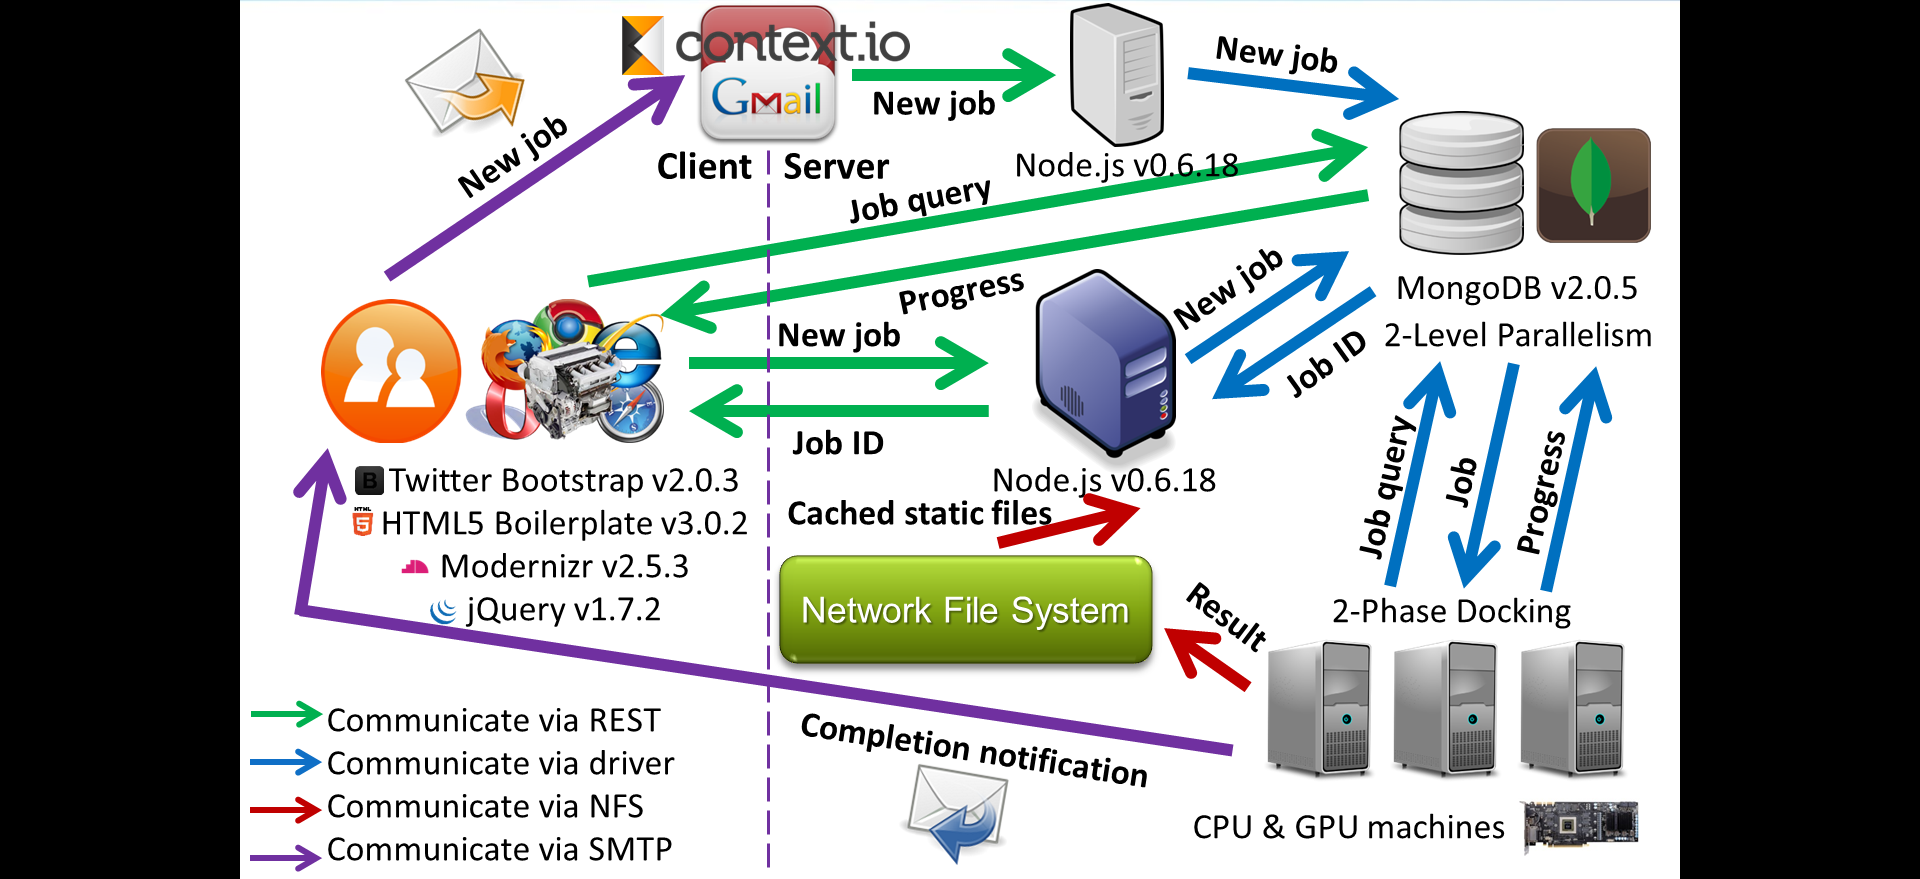
\includegraphics[width=\linewidth]{istar/Architecture.png}
\caption{istar architecture.}
\label{istar:Architecture}
\end{figure}

Figure \ref{istar:Website} shows istar web site. Job progress will be displayed in the upper section, while new jobs can be submitted in the lower section. A new job typically consists of several compulsory fields as well as several optional fields. Compulsory fields include a receptor in PDBQT format, a search space defined by a cubic box, a short job description, and an email to receive completion notification. Optional fields include 8 ligand filtering conditions, like molecular weight, partition coefficient clogP, number of hydrogen bond donors, number of hydrogen bond acceptors, number of rotatable bonds, polar surface area tPSA, apolar desolvation and polar desolvation. We set up default values for optional fields, and only the ZINC ligands satisfying all the 8 filtering conditions will be screened.

\begin{figure}
\centering
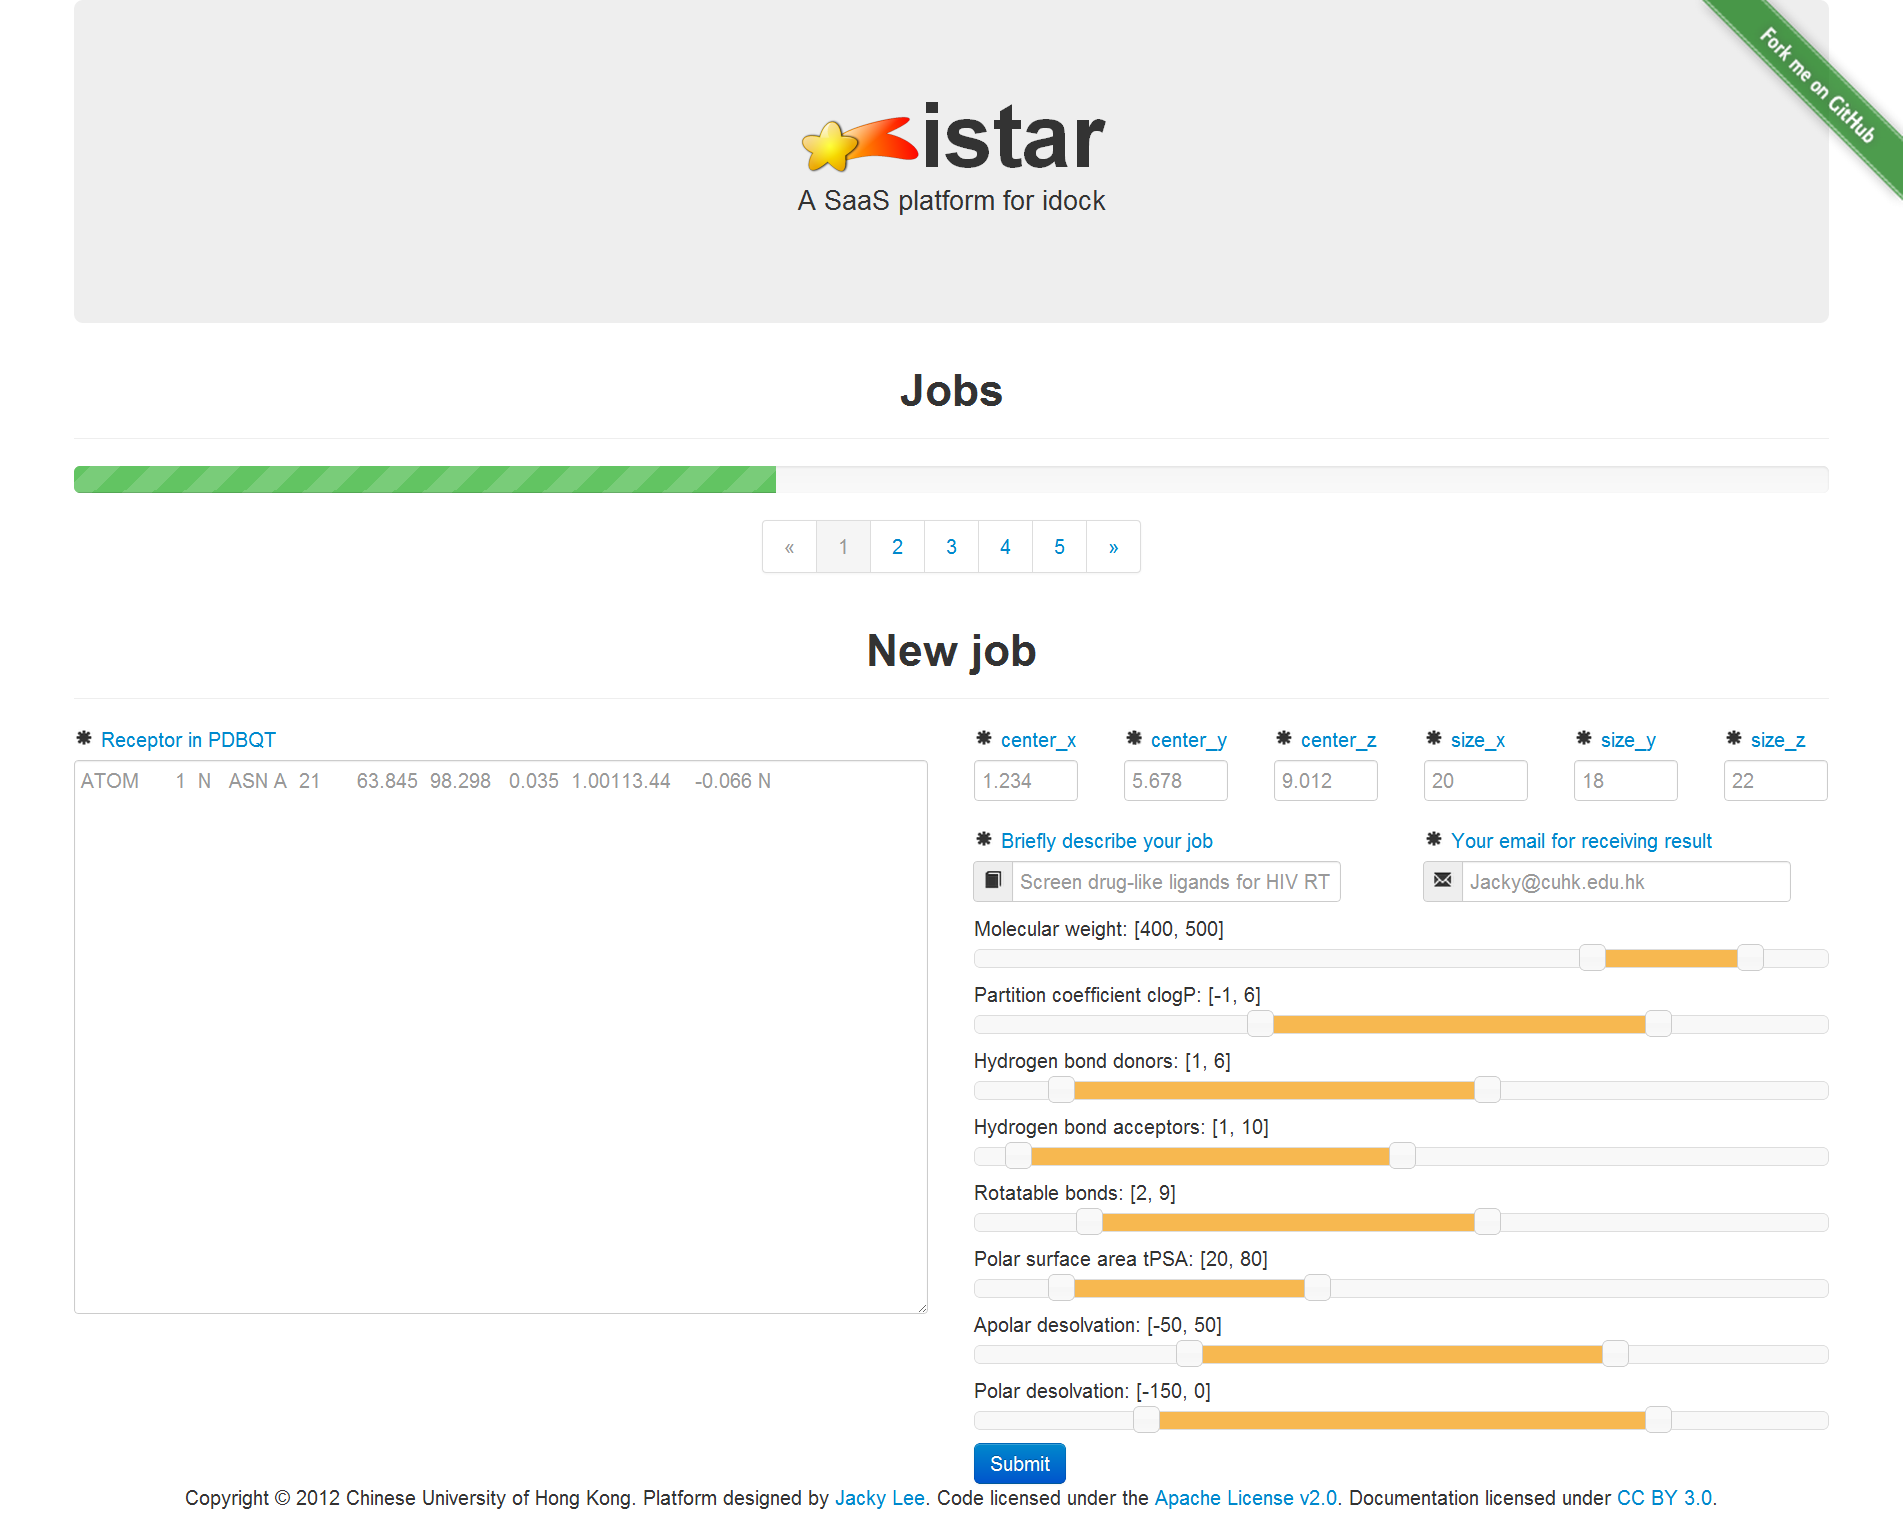
\includegraphics[width=\linewidth]{istar/Website.png}
\caption{istar web site.}
\label{istar:Website}
\end{figure}

istar features slice-level parallelism. Generally speaking, workstations can compete for jobs or slices, with the former known as job-level parallelism and the latter as slice-level parallelism (Figure \ref{istar:2LevelParallelism}). Job-level parallelism is very straightforward to implement and can ensure 100\% utilization of computational power when the number of jobs exceeds the number of workstations. Nevertheless, when the number of workstations exceeds the number of jobs, which is usually the case in practice during the initial stage of istar, slice-level parallelism can better utilize computational power by subdividing a job into 128 slices which are then distributed to workstations. Slice-level parallelism is, in contrast, difficult to implement. The technical hurdle becomes even more apparent when progress must be reported to MongoDB from time to time, and progresses from multiple slices must be combined to compute an overall progress.

\begin{figure}
\centering
\subfloat[Job-level parallelism.]
{
  \label{istar:JobLevelParallelism}
  
\includegraphics[width=\linewidth]{istar/JobLevelParallelism.png}
}
\\
\subfloat[Slice-level parallelism.]
{
  \label{istar:SliceLevelParallelism}
  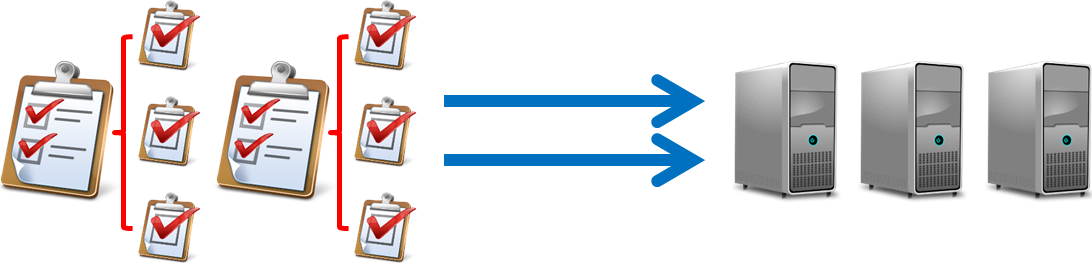
\includegraphics[width=\linewidth]{istar/SliceLevelParallelism.png}
}
\caption{istar 2-level parallelism.}
\label{istar:2LevelParallelism}
\end{figure}

istar features 2-phase docking, due to as many as 12 millions ligands to screen. In phase 1, idock performs coarse but fast virtual screening without writing any conformations to file, aiming to quickly shortlist a few candidate compounds. In phase 2, idock performs fine and slow virtual screening, writing as many conformations to file as possible, aiming to refine the predicted free energy of candidate compounds. Such a 2-phase docking methodology can significantly reduce job execution time while avoiding the risk of filtering out promising compounds, resulting in a low false negative rate.

\begin{figure}
\centering
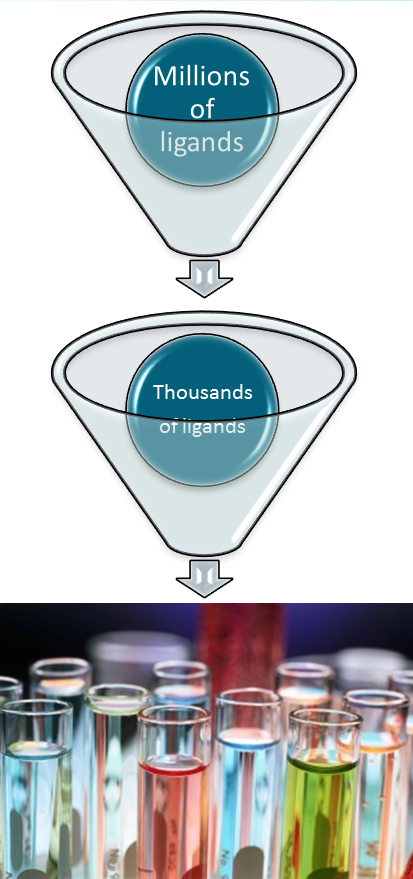
\includegraphics[width=\linewidth]{istar/2PhaseDocking.png}
\caption{istar 2-phase docking.}
\label{istar:2PhaseDocking}
\end{figure}

istar serves as our foundation for SaaS. With istar at hand, basically we can expose any of our software as a service. Once we manage to host idock at istar, it will be quite easy for us to host our other tools, such as igrow for computational synthesis of potent ligands.

As for software availability, similar to idock, istar is also hosted at GitHub for version control and freely available at http://github.com/HongjianLi/istar. Its source code is licensed under the Apache License 2.0 while its documentation is licensed under CC BY 3.0. A live demo will be available at http://istar.cse.cuhk.edu.hk when we finish implementing istar.

\section{idock 2.0: GPU Acceleration of idock}

Even though idock 1.4 outperformed AutoDock Vina by 10x in terms of docking speed, it still required about 10 hours on average to dock 10,928 drug-like ligands against a certain protein, not to mention massive docking of millions of ligands. Virtual screening remains a time-consuming practice. Faster implementations are highly desired.

We used AMD CodeAnalyst Performance Analyzer v3.6 to detect program hotspots and observe thread behaviors. Figure \ref{idock:ThreadProfile} shows the thread profile of idock 1.4. Thread 1060 was the main thread, while the other four were workers threads spawned by the main thread and maintained by our novel thread pool. During program startup, the main thread parsed command line arguments, initialized necessary variables, parsed receptor file, and created a thread pool to precalculate the scoring function in parallel. Afterwards, it entered a loop, docking ligands one by one. The four workers threads actually carried out the creation of grid maps as well as running Monte Carlo tasks in parallel, fully occupaying all the fours CPU cores. Upon completion of docking a ligand, the control was returned to the main thread to write conformations to file and read the next ligand from file. From the figure, it can be concluded that the precalculation of grid maps and the execution of Monte Carlo tasks constitute the program hotspots and the worker threads acquire most of the CPU computing resources.

\begin{figure}
\centering
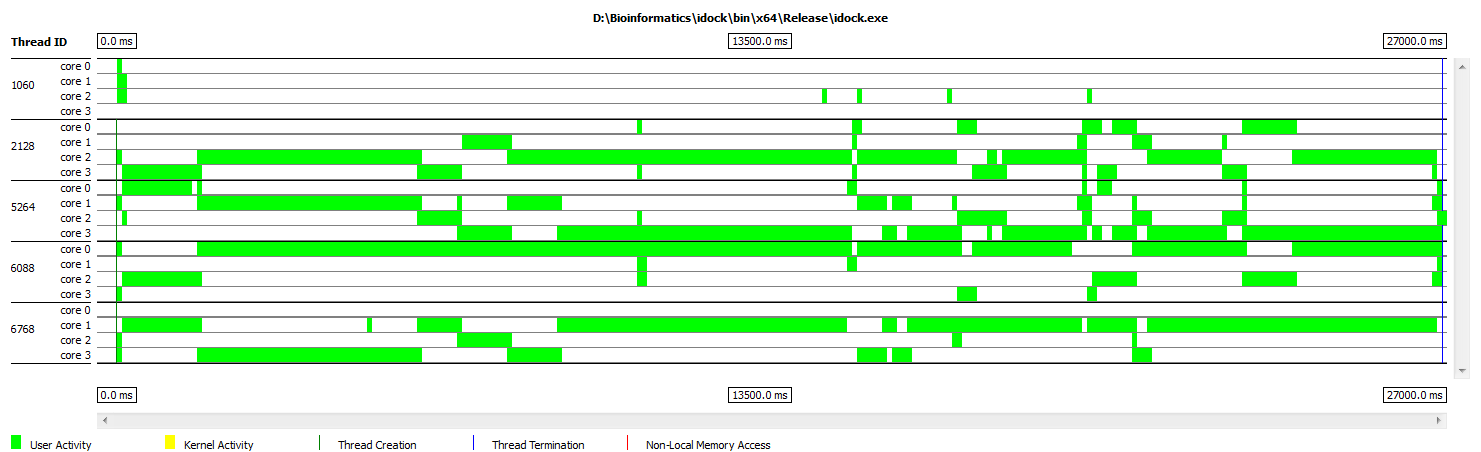
\includegraphics[width=\textwidth]{idock/ThreadProfile.png}
\caption{idock thread profile.}
\label{idock:ThreadProfile}
\end{figure}

We propose idock 2.0, incorporating GPU acceleration with both CUDA and OpenCL, harvesting the trenemdous computational power offered by modern GPUs nowadays. In \citeyear{1138} we developed a fast CUDA implementation of agrep algorithm for approximate nucleotide sequence matching \citep{1138}, demonstrating our expertise in CUDA programming.

Performance optimization revolves around three basic strategies: 1) maximizing parallel execution, 2) maximizing memory bandwidth, and 3) maximizing instruction throughput.

Maximizing parallel execution can be achieved by exposing as much data parallelism as possible and mapping the parallelism to the hardware as efficiently as possible. In dock, we have parallelized both the precalculation of grid maps and the Monte Carlo global optimization using our novel thread pool in order to utilize multicore CPU. We plan to port these two most time-consuming parts to the GPU, map Monte Carlo tasks directly to CUDA threads, and use the occupancy calculator to carefully choose the execution configuration of each kernel launch in order to maintain a high GPU utilization. Several technical difficulties exist. One difficulty is the lack of sufficient capacity of GDDR5 memory, which is merely 2 GB along with a GeForce GTX680. This voids the precalculation of grid maps at a fine granularity like 0.8 \AA, leading to reduced approximation accuracy and possibly a high false negative rate. Another difficulty is the efficient generation of pseudo random numbers. Although there is an official library for this purpose, it is hard to determine the number of random numbers in need in advance because the Monte Carlo algorithm is stochastic \textit{per se}.

Maximizing memory bandwidth can be achieved by minimizing data transfers between the host and the device and optimizing the access patterns to global memory and shared memory on the device. Since host-to-device and device-to-host data transfers have much lower bandwidth than internal device data transfers, we plan to accommodate as much data as possible into the GPU global memory. In idock 2.0, constant data such as structure of receptor, definition of search space, precalculation of scoring function, and some configurations for the BFGS Quasi-Newton optimizer will reside in constant cache, while grid maps, due to its huge size, will resize in global memory, and temporary variables will resize in per-thread registers.

Maximizing global memory bandwidth is of no.1 importance, and its bandwidth depends largely on its access pattern. Figure \ref{GPU:AlignedSequentialGlobalMemoryAccess} shows an example of aligned and sequential global memory access and corresponding memory transactions based on compute capability. In this case, threads of a warp access adjacent 4-byte words such as adjacent float values. In other words, the \textit{k}th thread accesses the \textit{k}th word in a 128B L1 cache line, a single coalesced transaction alone will service that memory access. In idock 2.0, we will adopt this kind of aligned and sequential access pattern and re-organize array of structures into structure of arrays, e.g.  [ \{ x1, y1, z1 \}, \{ x2, y2, z2 \} ] into \{ [ x1, x2 ], [ y1, y2 ], [ z1, z2 ] \}. Such a restructing requires rewriting almost all the relevant mathematical data structures and functions in use in idock. So far we have stepped towards this direction a little bit, finishing rewriting the templated quaternion class from the BOOST C++ library into our own light-weight version to represent the orientation of a conformation.

\begin{figure}
\centering
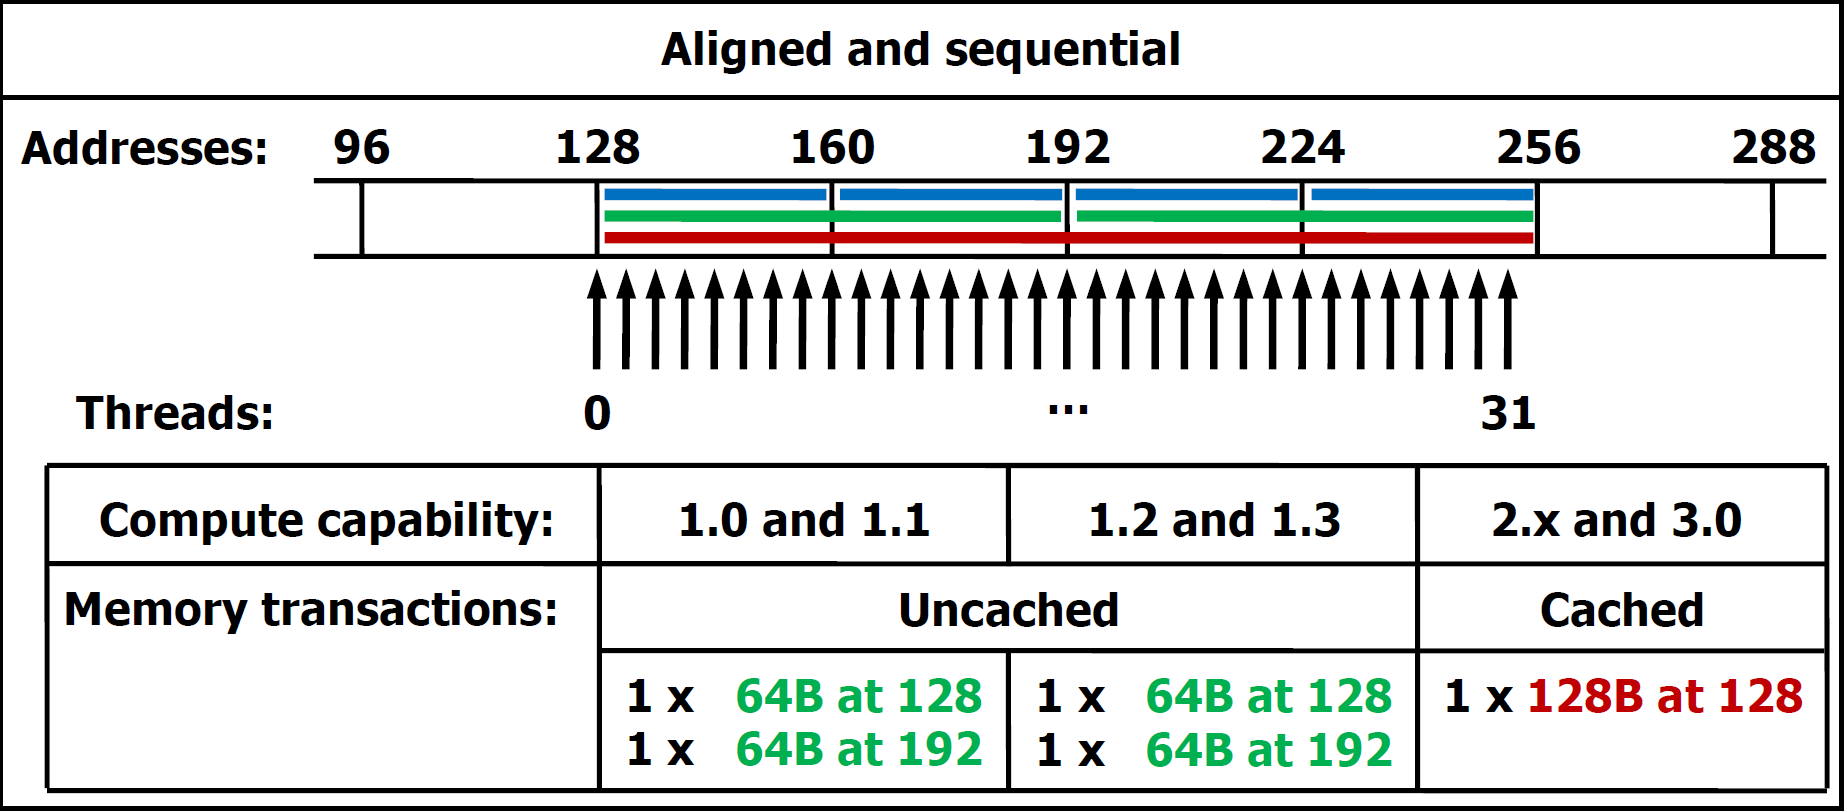
\includegraphics[width=\linewidth]{GPU/AlignedSequentialGlobalMemoryAccess.png}
\caption{Aligned and sequential global memory accesses by a warp, 4-byte word per thread, and associated memory transactions based on compute capability. Source: NVIDIA.}
\label{GPU:AlignedSequentialGlobalMemoryAccess}
\end{figure}

Each SMX has 64 KB of on-chip memory that can be configured as 48 KB of shared memory with 16 KB of L1 cache, or as 16 KB of shared memory with 48 KB of L1 cache. Since threads within a thread block run their Monte Carlo tasks independently and seldom communicate with one another, we decide to allocate 48 KB of the 64 KB on-chip memory to L1 cache.

Maximizing instruction throughput can be achieved by using single precision instead of double precision and using intrinsics instead of regular functions. This suggests trading precision for speed as long as the final result is not affected. Since most contemporary GPU chips supply with an astonishingly high throughput for single precision operations at TFLOP level but a relatively low throughput for double precision operations, we prefer the former. In order to make sure the precision loss must not affect the end result too much, we did an in-house trial, demoting double to float in idock 1.4, only to find that the predicted conformation and free energy were exactly identical as in the case of double precision given the same random seed for initializing the pseudo random number generator. This experiment concluded idock to be insensitive to precision switch and it is thus safe enough to utilize single precision operations as well as intrinsics in idock 2.0.

\section{igrow: Click Chemistry for idock}

In 2011, inspired by AutoGrow \citep{466}, we developed SmartGrow, addressing several problems that AutoGrow suffers from.

It inherits the mutation and crossover operators from AutoGrow. igrow implements Lipinski's \textit{Rule of Five} \citep{168} to ensure drug likeness. The program design is so flexible that it reserves room for adaptation to new chemical constraints. Its robust parser correctly processes two-letter chemical elements, and meanwhile adds additional support for phosphorus.

SmartGrow helped to explore a much larger chemical space for novel drugs. It displayed comparable performance in terms of predicted free energy but outperforms AutoGrow by 30\% in terms of execution time on average across 18 test cases. Ligands generated by SmartGrow retained molecular weights 100 Da lower than AutoGrow and never exceed 500 Da so that they can be absorbed by human body. 

However, we wrote SmartGrow in a hurry and did not follow a formal software engineering approach. Later on when we conducted a benchmark on SmartGrow, we discovered a great many of exceptional bugs that were very hard to fix due to the messy code structure. Regretfully, we decided to abandon the buggy SmartGrow.

We propose igrow as a successor SmartGrow. We rewrote igrow from scratch, carefully examining each line of code in a systematic manner.

Figure \ref{igrow:ComputationalSynthesis} shows the relationship between igrow and idock.

Exactly because of the close relationship between igrow and idock, igrow borrowed several great ideas from idock. igrow invents its own thread pool in order to reuse threads and maintain a high CPU utilization throughout the entire screening procedure. The thread pool parallelizes the execution of mutation and crossover operators. igrow estimates the capacity of every vector structure and intensively utilizes Rvalue reference, a new feature in the C++11 standard, to avoid frequent memory reallocation. igrow accelerates the assignment of atom types by making use of residue information for receptor and branch information for ligand, without explicitly detecting covalent bonds among atoms.

\begin{figure}
\centering
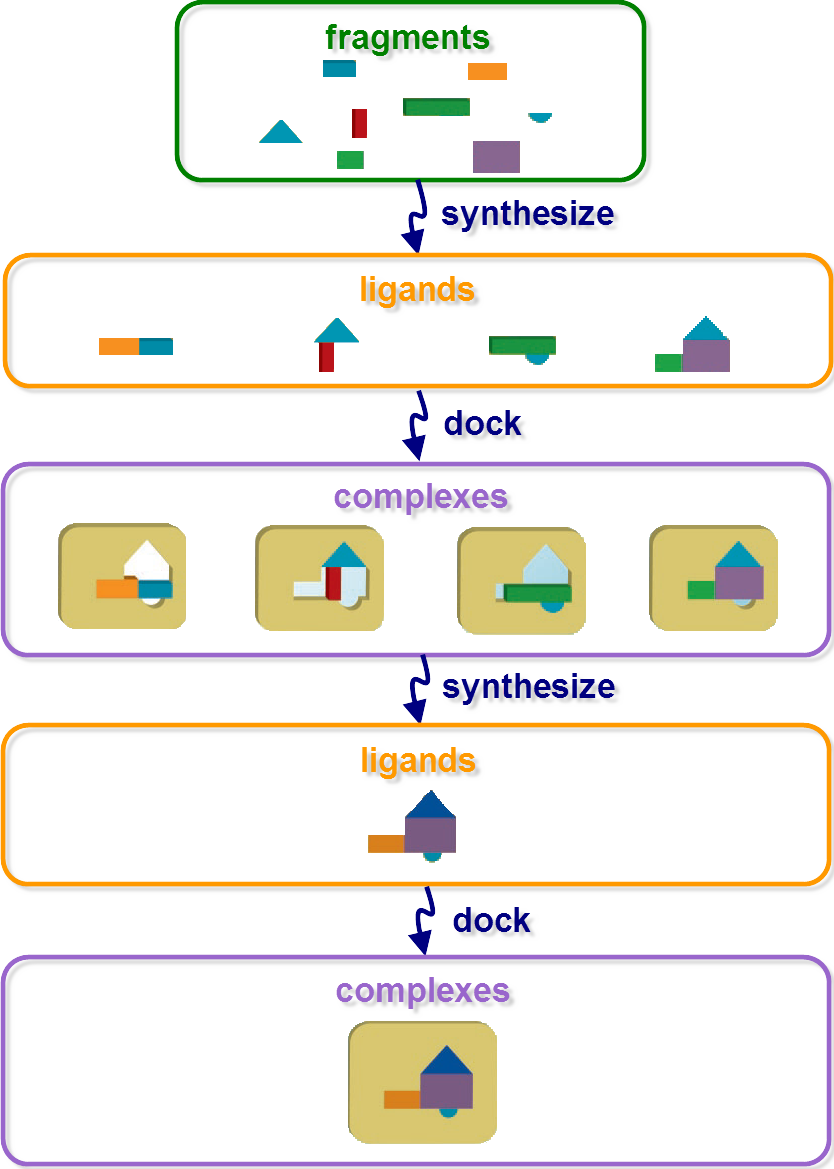
\includegraphics[width=\textwidth]{igrow/ComputationalSynthesis.png}
\caption{Iteratively synthesizing novel ligands from fragments with igrow followed by docking with idock.}
\label{igrow:ComputationalSynthesis}
\end{figure}

Figure \ref{igrow:Flowchart} shows the flowchart of current implementation of igrow. 

\begin{figure}
\centering
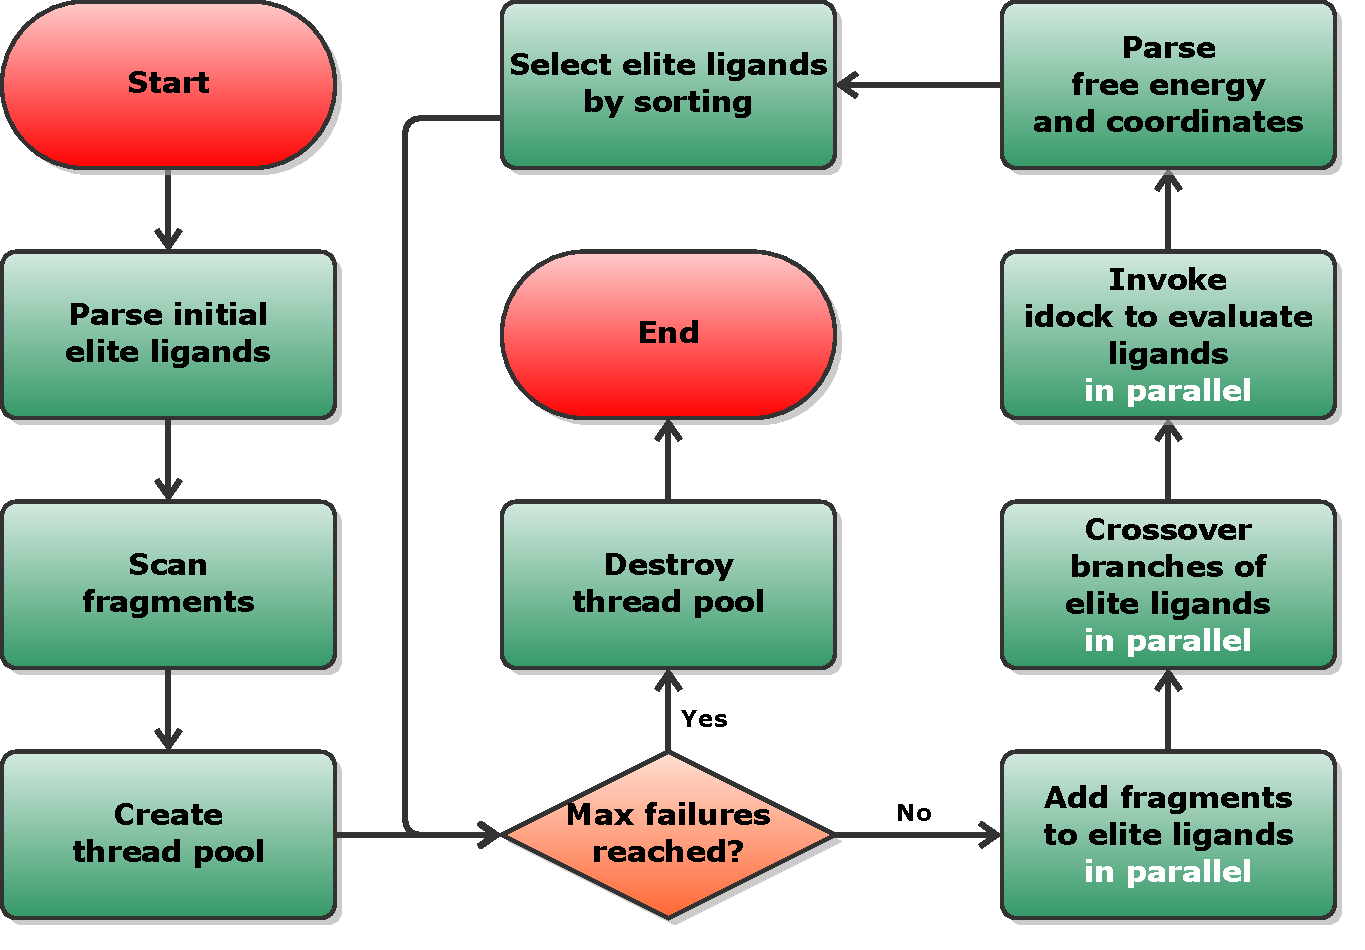
\includegraphics[width=\textwidth]{igrow/Flowchart.pdf}
\caption{igrow flowchart.}
\label{igrow:Flowchart}
\end{figure}

Future work, 1) click chemistry, 2) integration.
We will try to integrate igrow into idock to realize grid map caching as well as partial docking.
 
As for software availability, igrow is free and open source under Apache License 2.0. It is written in C++ and available at http://github.com/HongjianLi/igrow. Precompiled executables for 32-bit and 64-bit Linux, Windows, Mac OS X, FreeBSD and Solaris are provided. Docking examples and API documentations are also provided.

\section{ADMET Property Prediction}

It was estimated that 40\% to 60\% of new chemical entity (NCE) failures can be attributed to poor ADMET (absorption, distribution, metabolism, excretion, and toxicity) profiles.

PKKB (PharmacoKinetics Knowledge Base) \citep{1133} provides the most extensive collection of freely available data for ADMET properties up to date. PKKB integrates 31,412 experimental or predicted values for 1,685 drug and drug-like molecules from published literature with available experimental ADMET properties including partition coefficient (logP), solubility (logS), intestinal absorption, Caco-2 permeability, human bioavailability, plasma protein binding, volume of distribution, distribution of blood, half-time, excretion, urinary excretion, clearance, toxicity, etc. (Table \ref{PKKB:Properties})

\begin{table}
\centering
\begin{tabular*}
{\linewidth}
{@{\extracolsep{\fill}}rlr}
\toprule
No. & Property & Measurements \\
\midrule
\multicolumn{3}{l}{\textbf{Molecular properties}}\\
1 & Molecular weight & 1,684 \\
2 & logP (experiment) & 1,019 \\
3 & logP (predicted, AB/logP v2.0) & 1,625 \\
4 & Pka & 638 \\
5 & logD (pH=7,predicted) & 1,625 \\
6 & Solubility (experiment) & 800 \\
7 & logS (predicted, ACD/Labs)(pH=7) & 1,614 \\
8 & logSw (predicted, AB/LogSw 2.0) & 1,625 \\
9 & Sw (mg/ml) (predicted, ACD/Labs) & 1,613 \\
10 & Sw (predicted) & 1,625 \\
11 & No. of hbond donors & 1,625 \\
12 & No. of hbond acceptors & 1,625 \\
13 & No. of rotatable bonds & 1,625 \\
14 & TPSA & 1,625 \\
\noalign{\smallskip\smallskip}
\multicolumn{3}{l}{\textbf{Pharmacology}}\\
15 & Status & 1,372 \\
16 & Administration & 501 \\
17 & Pharmacology & 1,543 \\
\noalign{\smallskip\smallskip}
\multicolumn{3}{l}{\textbf{Absorption}}\\
18 & Intestinal absorption & 679 \\
19 & Absorption (description) & 699 \\
20 & Caco-2 & 64 \\
21 & Human bioavailability & 992 \\
\noalign{\smallskip\smallskip}
\multicolumn{3}{l}{\textbf{Distribution}}\\
22 & Plasma protein binding & 1058 \\
23 & Volume of distribution(Vd) & 646 \\
24 & D-blood & 66 \\
\noalign{\smallskip\smallskip}
\multicolumn{3}{l}{\textbf{Metabolism}}\\
25 & Metabolism & 1,111 \\
26 & Half-time & 1,116 \\
\noalign{\smallskip\smallskip}
\multicolumn{3}{l}{\textbf{Excretion}}\\
27 & Excretion & 855 \\
28 & Urinary excretion & 281 \\
29 & Clearance & 410 \\
\noalign{\smallskip\smallskip}
\multicolumn{3}{l}{\textbf{Toxicity}}\\
30 & Toxicity & 873 \\
31 & LD50 (rat) & 219 \\
32 & LD50 (mouse) & 243 \\
\bottomrule
\end{tabular*}
\caption{PKKB property measurements.}
\label{PKKB:Properties}
\end{table}

Figure \ref{PKKB:Schema} shows the PKKB schema. Raw data from literature was first converted into proper formats and then integrated into a central ADMET database. A web site is provided for interactive search of ADMET properties given either structure or descriptive text of compounds of interest.

\begin{figure}
\centering
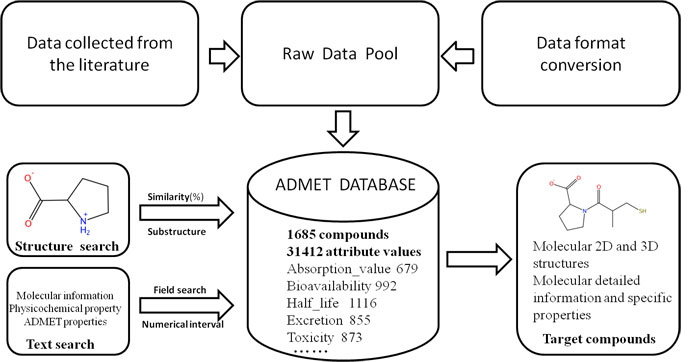
\includegraphics[width=\linewidth]{PKKB/Schema.jpg}
\caption{PKKB schema.}
\label{PKKB:Schema}
\end{figure}

Thanks to the availability of reliable experimental data and basic structural information from PKKB enables, \textit{in silico} ADMET modeling becomes viable. One can predict ADMET properties from chemical structures for a huge number of compounds without actually synthesizing or assaying them.

We propose to make use of advanced machine learning techniques to train a regression model (Figure \ref{PKKB:Regression}), be it linear or non-linear. Once the model is constructed, it is possible to predict ADMET properties of any given compounds. Coupled with conformations and free energy predicted by our tool idock, we can better evaluate a compound from a wide variety of perspectives, leading to a higher drug discovery success rate. Moreover, such a regression model can be integrated into igrow to guide ligand synthesis, which can then be further integrated into idock to guide ligand filtering and eventually into istar to compose a comprehensive framework for structure-based drug discovery.

\begin{figure}
\centering
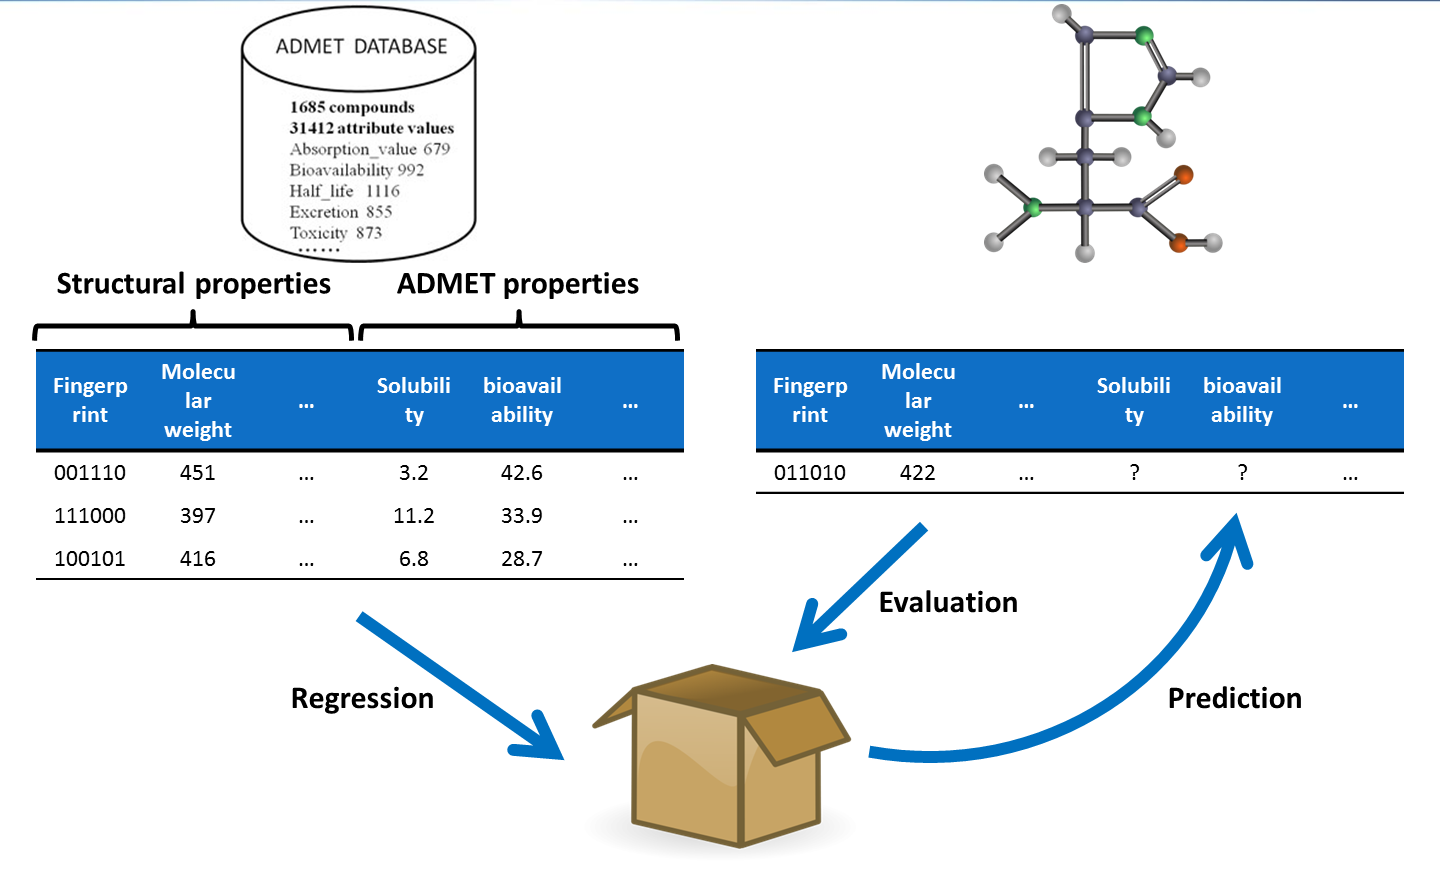
\includegraphics[width=\linewidth]{PKKB/Regression.png}
\caption{Our proposed regression model for PKKB.}
\label{PKKB:Regression}
\end{figure}

\section{Real-Life Drug Discovery Case Studies}

Our colleges and collaborators as biochemists and pharmacists are working on several high-impact drug discovery projects. They have done lots of biological assays and succeeded in identifying pharmaceutical and druggable protein targets for certain diseases. They outsource the docking tasks to us, hoping to discover potent and selective inhibitors of certain proteins.

Prof. P.C. Shaw from School of Life Sciences at Chinese University of Hong Kong has studied Influenza A H1N1 for years. (2IQH, 2ZNL)

Prof. Marie Chia-Mi Lin from Department of Surgery at Prince of Wales Hospital has studied CCRK for years. (1HCL)

Dr. Hong Yao from School of Public Health \& Primary Care at Chinese University of Hong Kong, cancer stem cell Wnt (1GTE), 

\chapterend
